\documentclass[twoside]{book}

% Packages required by doxygen
\usepackage{fixltx2e}
\usepackage{calc}
\usepackage{doxygen}
\usepackage[export]{adjustbox} % also loads graphicx
\usepackage{graphicx}
\usepackage[utf8]{inputenc}
\usepackage{makeidx}
\usepackage{multicol}
\usepackage{multirow}
\PassOptionsToPackage{warn}{textcomp}
\usepackage{textcomp}
\usepackage[nointegrals]{wasysym}
\usepackage[table]{xcolor}

% Font selection
\usepackage[T1]{fontenc}
\usepackage[scaled=.90]{helvet}
\usepackage{courier}
\usepackage{amssymb}
\usepackage{sectsty}
\renewcommand{\familydefault}{\sfdefault}
\allsectionsfont{%
  \fontseries{bc}\selectfont%
  \color{darkgray}%
}
\renewcommand{\DoxyLabelFont}{%
  \fontseries{bc}\selectfont%
  \color{darkgray}%
}
\newcommand{\+}{\discretionary{\mbox{\scriptsize$\hookleftarrow$}}{}{}}

% Page & text layout
\usepackage{geometry}
\geometry{%
  a4paper,%
  top=2.5cm,%
  bottom=2.5cm,%
  left=2.5cm,%
  right=2.5cm%
}
\tolerance=750
\hfuzz=15pt
\hbadness=750
\setlength{\emergencystretch}{15pt}
\setlength{\parindent}{0cm}
\setlength{\parskip}{0.2cm}
\makeatletter
\renewcommand{\paragraph}{%
  \@startsection{paragraph}{4}{0ex}{-1.0ex}{1.0ex}{%
    \normalfont\normalsize\bfseries\SS@parafont%
  }%
}
\renewcommand{\subparagraph}{%
  \@startsection{subparagraph}{5}{0ex}{-1.0ex}{1.0ex}{%
    \normalfont\normalsize\bfseries\SS@subparafont%
  }%
}
\makeatother

% Headers & footers
\usepackage{fancyhdr}
\pagestyle{fancyplain}
\fancyhead[LE]{\fancyplain{}{\bfseries\thepage}}
\fancyhead[CE]{\fancyplain{}{}}
\fancyhead[RE]{\fancyplain{}{\bfseries\leftmark}}
\fancyhead[LO]{\fancyplain{}{\bfseries\rightmark}}
\fancyhead[CO]{\fancyplain{}{}}
\fancyhead[RO]{\fancyplain{}{\bfseries\thepage}}
\fancyfoot[LE]{\fancyplain{}{}}
\fancyfoot[CE]{\fancyplain{}{}}
\fancyfoot[RE]{\fancyplain{}{\bfseries\scriptsize Generated on Sat May 23 2015 11\+:16\+:30 for Mosaic Morphing by Doxygen }}
\fancyfoot[LO]{\fancyplain{}{\bfseries\scriptsize Generated on Sat May 23 2015 11\+:16\+:30 for Mosaic Morphing by Doxygen }}
\fancyfoot[CO]{\fancyplain{}{}}
\fancyfoot[RO]{\fancyplain{}{}}
\renewcommand{\footrulewidth}{0.4pt}
\renewcommand{\chaptermark}[1]{%
  \markboth{#1}{}%
}
\renewcommand{\sectionmark}[1]{%
  \markright{\thesection\ #1}%
}

% Indices & bibliography
\usepackage{natbib}
\usepackage[titles]{tocloft}
\setcounter{tocdepth}{3}
\setcounter{secnumdepth}{5}
\makeindex

% Hyperlinks (required, but should be loaded last)
\usepackage{ifpdf}
\ifpdf
  \usepackage[pdftex,pagebackref=true]{hyperref}
\else
  \usepackage[ps2pdf,pagebackref=true]{hyperref}
\fi
\hypersetup{%
  colorlinks=true,%
  linkcolor=blue,%
  citecolor=blue,%
  unicode%
}

% Custom commands
\newcommand{\clearemptydoublepage}{%
  \newpage{\pagestyle{empty}\cleardoublepage}%
}


%===== C O N T E N T S =====

\begin{document}

% Titlepage & ToC
\hypersetup{pageanchor=false,
             bookmarks=true,
             bookmarksnumbered=true,
             pdfencoding=unicode
            }
\pagenumbering{roman}
\begin{titlepage}
\vspace*{7cm}
\begin{center}%
{\Large Mosaic Morphing }\\
\vspace*{1cm}
{\large Generated by Doxygen 1.8.9.1}\\
\vspace*{0.5cm}
{\small Sat May 23 2015 11:16:30}\\
\end{center}
\end{titlepage}
\clearemptydoublepage
\tableofcontents
\clearemptydoublepage
\pagenumbering{arabic}
\hypersetup{pageanchor=true}

%--- Begin generated contents ---
\chapter{Hierarchical Index}
\section{Class Hierarchy}
This inheritance list is sorted roughly, but not completely, alphabetically\+:\begin{DoxyCompactList}
\item Q\+G\+L\+Widget\begin{DoxyCompactList}
\item \contentsline{section}{G\+L\+Widget}{\pageref{class_g_l_widget}}{}
\end{DoxyCompactList}
\item Q\+Main\+Window\begin{DoxyCompactList}
\item \contentsline{section}{Main\+Window}{\pageref{class_main_window}}{}
\end{DoxyCompactList}
\item \contentsline{section}{Tile}{\pageref{class_tile}}{}
\end{DoxyCompactList}

\chapter{Class Index}
\section{Class List}
Here are the classes, structs, unions and interfaces with brief descriptions\+:\begin{DoxyCompactList}
\item\contentsline{section}{\hyperlink{class_g_l_widget}{G\+L\+Widget} }{\pageref{class_g_l_widget}}{}
\item\contentsline{section}{\hyperlink{class_main_window}{Main\+Window} }{\pageref{class_main_window}}{}
\item\contentsline{section}{\hyperlink{class_tile}{Tile} }{\pageref{class_tile}}{}
\end{DoxyCompactList}

\chapter{Class Documentation}
\hypertarget{class_g_l_widget}{}\section{G\+L\+Widget Class Reference}
\label{class_g_l_widget}\index{G\+L\+Widget@{G\+L\+Widget}}
Inheritance diagram for G\+L\+Widget\+:\begin{figure}[H]
\begin{center}
\leavevmode
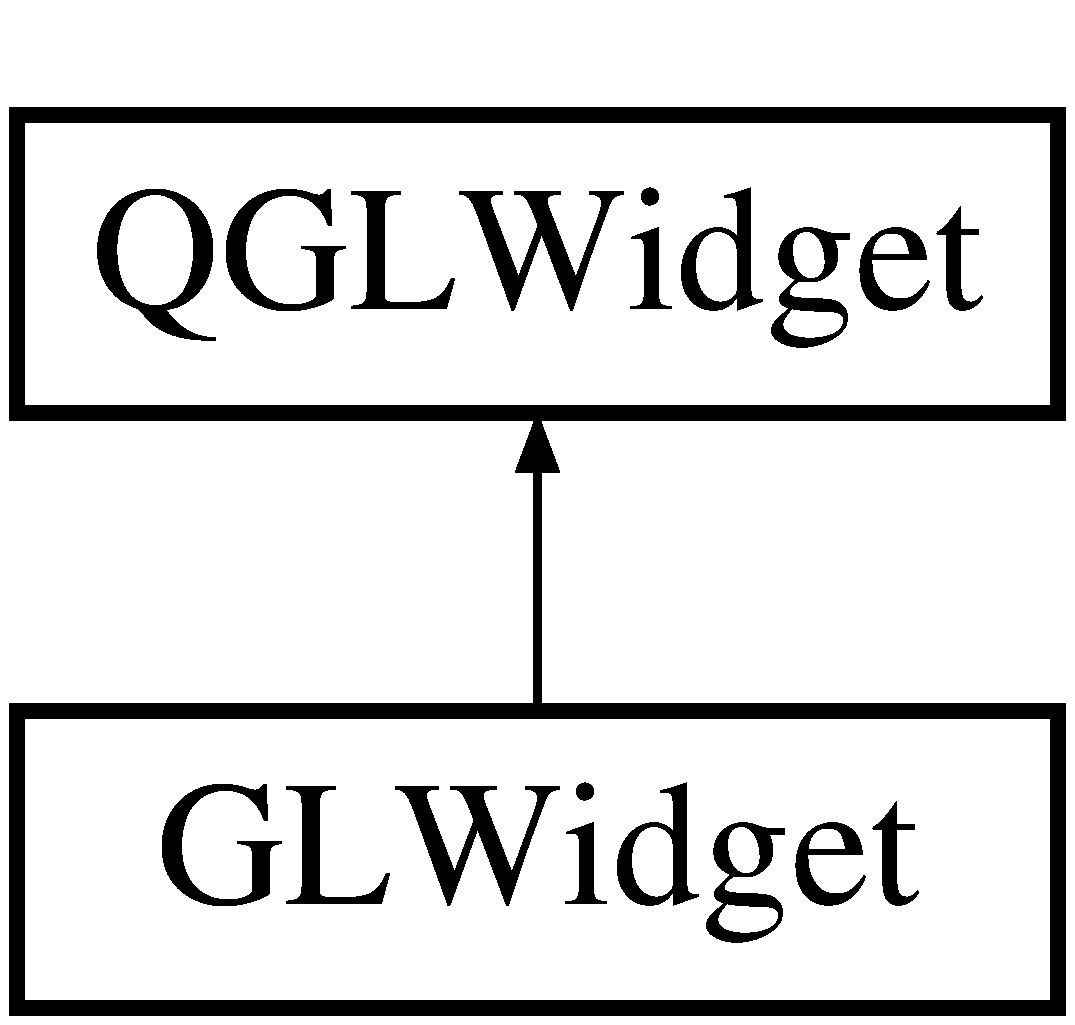
\includegraphics[height=2.000000cm]{class_g_l_widget}
\end{center}
\end{figure}
\subsection*{Public Slots}
\begin{DoxyCompactItemize}
\item 
\hypertarget{class_g_l_widget_a7ac160de2da0aa3d6ca2fbe8ac9be34b}{}void \hyperlink{class_g_l_widget_a7ac160de2da0aa3d6ca2fbe8ac9be34b}{s\+\_\+set\+Scale} (int flag)\label{class_g_l_widget_a7ac160de2da0aa3d6ca2fbe8ac9be34b}

\begin{DoxyCompactList}\small\item\em Slot function for setting the scale flag. \end{DoxyCompactList}\item 
\hypertarget{class_g_l_widget_a20fd67b0517c73ce404ef23c9fcb5e1d}{}void \hyperlink{class_g_l_widget_a20fd67b0517c73ce404ef23c9fcb5e1d}{s\+\_\+set\+Rotate} (int flag)\label{class_g_l_widget_a20fd67b0517c73ce404ef23c9fcb5e1d}

\begin{DoxyCompactList}\small\item\em Slot function for setting the rotate flag. \end{DoxyCompactList}\item 
\hypertarget{class_g_l_widget_a090fcf2a1e3ae0e462d89a72f279ac5a}{}void \hyperlink{class_g_l_widget_a090fcf2a1e3ae0e462d89a72f279ac5a}{s\+\_\+set\+Centroid} (int flag)\label{class_g_l_widget_a090fcf2a1e3ae0e462d89a72f279ac5a}

\begin{DoxyCompactList}\small\item\em Slot function for setting the centroid flag. \end{DoxyCompactList}\item 
\hypertarget{class_g_l_widget_accdba4e48f14b4b0872f2b39f2659b47}{}void \hyperlink{class_g_l_widget_accdba4e48f14b4b0872f2b39f2659b47}{s\+\_\+set\+Speed} (int speed)\label{class_g_l_widget_accdba4e48f14b4b0872f2b39f2659b47}

\begin{DoxyCompactList}\small\item\em Slot function for setting the animation speed. \end{DoxyCompactList}\item 
\hypertarget{class_g_l_widget_ada232e9c245b736f23a7f82b6d5d2ad0}{}void \hyperlink{class_g_l_widget_ada232e9c245b736f23a7f82b6d5d2ad0}{s\+\_\+play} ()\label{class_g_l_widget_ada232e9c245b736f23a7f82b6d5d2ad0}

\begin{DoxyCompactList}\small\item\em Slot function for playing/pausing the animation. \end{DoxyCompactList}\item 
\hypertarget{class_g_l_widget_a8820beb590afc1fd5709295a76d908a7}{}void \hyperlink{class_g_l_widget_a8820beb590afc1fd5709295a76d908a7}{s\+\_\+spiral} ()\label{class_g_l_widget_a8820beb590afc1fd5709295a76d908a7}

\begin{DoxyCompactList}\small\item\em Slot function for spiral effect. \end{DoxyCompactList}\item 
\hypertarget{class_g_l_widget_a5a6ff71edf2aa3dd064da7fe688fad0a}{}void \hyperlink{class_g_l_widget_a5a6ff71edf2aa3dd064da7fe688fad0a}{s\+\_\+space} ()\label{class_g_l_widget_a5a6ff71edf2aa3dd064da7fe688fad0a}

\begin{DoxyCompactList}\small\item\em Slot to control scale space. \end{DoxyCompactList}\item 
void \hyperlink{class_g_l_widget_ab82b7ae2912130fc5c990da90a75d19b}{s\+\_\+reset} ()
\begin{DoxyCompactList}\small\item\em Reset slot reinitializes initial values. \end{DoxyCompactList}\item 
\hypertarget{class_g_l_widget_a7083404e9ab8feffb2c486f7c15308ce}{}void {\bfseries set\+X\+Rotation} (int angle)\label{class_g_l_widget_a7083404e9ab8feffb2c486f7c15308ce}

\item 
\hypertarget{class_g_l_widget_a29012eba3cb4201f78807066f2c9dcd4}{}void {\bfseries set\+Y\+Rotation} (int angle)\label{class_g_l_widget_a29012eba3cb4201f78807066f2c9dcd4}

\item 
\hypertarget{class_g_l_widget_a6f6b4fbbcc566d999db7e53aadeba889}{}void {\bfseries set\+Z\+Rotation} (int angle)\label{class_g_l_widget_a6f6b4fbbcc566d999db7e53aadeba889}

\end{DoxyCompactItemize}
\subsection*{Signals}
\begin{DoxyCompactItemize}
\item 
\hypertarget{class_g_l_widget_a3a557b9cd96f7b89661ceaa567c91640}{}void {\bfseries x\+Rotation\+Changed} (int angle)\label{class_g_l_widget_a3a557b9cd96f7b89661ceaa567c91640}

\item 
\hypertarget{class_g_l_widget_ad47d672d0124b995e82551a95b59badb}{}void {\bfseries y\+Rotation\+Changed} (int angle)\label{class_g_l_widget_ad47d672d0124b995e82551a95b59badb}

\item 
\hypertarget{class_g_l_widget_ab2035753b19b46105020d6045ac75a79}{}void {\bfseries z\+Rotation\+Changed} (int angle)\label{class_g_l_widget_ab2035753b19b46105020d6045ac75a79}

\end{DoxyCompactItemize}
\subsection*{Public Member Functions}
\begin{DoxyCompactItemize}
\item 
\hypertarget{class_g_l_widget_ab79c391c86de1ffb76f6950b49d82c0c}{}{\bfseries G\+L\+Widget} (Q\+Widget $\ast$parent=0)\label{class_g_l_widget_ab79c391c86de1ffb76f6950b49d82c0c}

\item 
\hypertarget{class_g_l_widget_a8faaa1bdf86f983888fcb40d9d8ac299}{}void {\bfseries set\+Tiles} (vector$<$ \hyperlink{class_tile}{Tile} $>$ \&)\label{class_g_l_widget_a8faaa1bdf86f983888fcb40d9d8ac299}

\item 
void \hyperlink{class_g_l_widget_ac615f919f588064feead6d7121a2c69a}{draw\+Tiles} ()
\begin{DoxyCompactList}\small\item\em Draw\+Tiles rotating/scaled tile animation. \end{DoxyCompactList}\item 
\hypertarget{class_g_l_widget_a1db972c9e72bb07a0266db84bc05576e}{}void {\bfseries set\+Timer} ()\label{class_g_l_widget_a1db972c9e72bb07a0266db84bc05576e}

\item 
void \hyperlink{class_g_l_widget_a3c710ff5b57368382b11c169d393c9b8}{radial\+Motion} (\hyperlink{class_tile}{Tile} \&)
\begin{DoxyCompactList}\small\item\em Update the depth and angles of tiles. \end{DoxyCompactList}\item 
\hypertarget{class_g_l_widget_ad1464ede635f26dddb3751d9e198e1a9}{}Q\+Vector3\+D {\bfseries compute\+Normal} (Q\+Vector2\+D \&, Q\+Vector2\+D \&, float, float)\label{class_g_l_widget_ad1464ede635f26dddb3751d9e198e1a9}

\item 
\hypertarget{class_g_l_widget_a6083f12756d3efaa54552ac7d77e543b}{}void {\bfseries load\+Tiles} (Q\+String \&)\label{class_g_l_widget_a6083f12756d3efaa54552ac7d77e543b}

\item 
\hypertarget{class_g_l_widget_acc3d674e13bcc75f0de5c238957871f3}{}void \hyperlink{class_g_l_widget_acc3d674e13bcc75f0de5c238957871f3}{load\+Texture} ()\label{class_g_l_widget_acc3d674e13bcc75f0de5c238957871f3}

\begin{DoxyCompactList}\small\item\em \hyperlink{class_g_l_widget_acc3d674e13bcc75f0de5c238957871f3}{G\+L\+Widget\+::load\+Texture} gl\+Gen\+Textures(num,\&textarray) is used to generate the texture. Arguments are number of textures and the texture array. \end{DoxyCompactList}\item 
\hypertarget{class_g_l_widget_a12b6753a8d9d1eadc15989210d70a399}{}void {\bfseries load\+Texture1} ()\label{class_g_l_widget_a12b6753a8d9d1eadc15989210d70a399}

\end{DoxyCompactItemize}
\subsection*{Protected Member Functions}
\begin{DoxyCompactItemize}
\item 
\hypertarget{class_g_l_widget_a7fab13e8cc9fc0730ca54c08b2c923a7}{}void {\bfseries initialize\+G\+L} ()\label{class_g_l_widget_a7fab13e8cc9fc0730ca54c08b2c923a7}

\item 
\hypertarget{class_g_l_widget_a640b5570cb2b37724fd5b58a77339c5e}{}void {\bfseries paint\+G\+L} ()\label{class_g_l_widget_a640b5570cb2b37724fd5b58a77339c5e}

\item 
\hypertarget{class_g_l_widget_ac0d2a8ecf60907a81c0d73475d851025}{}void {\bfseries resize\+G\+L} (int width, int height)\label{class_g_l_widget_ac0d2a8ecf60907a81c0d73475d851025}

\item 
void \hyperlink{class_g_l_widget_ab144cc8064c1bbf6d0ef0646ca0bd06c}{mouse\+Press\+Event} (Q\+Mouse\+Event $\ast$event)
\item 
void \hyperlink{class_g_l_widget_a9043bac13d6f0a5307ea5c7f9b3caa50}{mouse\+Move\+Event} (Q\+Mouse\+Event $\ast$event)
\end{DoxyCompactItemize}


\subsection{Member Function Documentation}
\hypertarget{class_g_l_widget_ac615f919f588064feead6d7121a2c69a}{}\index{G\+L\+Widget@{G\+L\+Widget}!draw\+Tiles@{draw\+Tiles}}
\index{draw\+Tiles@{draw\+Tiles}!G\+L\+Widget@{G\+L\+Widget}}
\subsubsection[{draw\+Tiles}]{\setlength{\rightskip}{0pt plus 5cm}void G\+L\+Widget\+::draw\+Tiles (
\begin{DoxyParamCaption}
{}
\end{DoxyParamCaption}
)}\label{class_g_l_widget_ac615f919f588064feead6d7121a2c69a}


Draw\+Tiles rotating/scaled tile animation. 

Draw the tiles starting with gl\+Begin using G\+L\+\_\+\+P\+O\+L\+Y\+G\+O\+N\+S to draw rectangular prism tiles. Then gl\+Vertex3f--for xyz floats (3dimensional). Next the texture is implemented and close with gl\+End. Implements when m\+\_\+spiral is set true by checkbox. Implements spacing effect when m\+\_\+space is set true by checkbox. Calls radial motion effect in order to explode implode. Within the gl\+Push\+Matrix() and gl\+Pop\+Matrix() there is a translate, rotate, scale, and then translate back. This is to rotate and scale the tiles about their centroids. \hypertarget{class_g_l_widget_a9043bac13d6f0a5307ea5c7f9b3caa50}{}\index{G\+L\+Widget@{G\+L\+Widget}!mouse\+Move\+Event@{mouse\+Move\+Event}}
\index{mouse\+Move\+Event@{mouse\+Move\+Event}!G\+L\+Widget@{G\+L\+Widget}}
\subsubsection[{mouse\+Move\+Event}]{\setlength{\rightskip}{0pt plus 5cm}void G\+L\+Widget\+::mouse\+Move\+Event (
\begin{DoxyParamCaption}
\item[{Q\+Mouse\+Event $\ast$}]{event}
\end{DoxyParamCaption}
)\hspace{0.3cm}{\ttfamily [protected]}}\label{class_g_l_widget_a9043bac13d6f0a5307ea5c7f9b3caa50}
\hyperlink{class_g_l_widget}{G\+L\+Widget} mouse\+Move\+Event Updates x and y coordinates and allocates left or else right click and movement. \hypertarget{class_g_l_widget_ab144cc8064c1bbf6d0ef0646ca0bd06c}{}\index{G\+L\+Widget@{G\+L\+Widget}!mouse\+Press\+Event@{mouse\+Press\+Event}}
\index{mouse\+Press\+Event@{mouse\+Press\+Event}!G\+L\+Widget@{G\+L\+Widget}}
\subsubsection[{mouse\+Press\+Event}]{\setlength{\rightskip}{0pt plus 5cm}void G\+L\+Widget\+::mouse\+Press\+Event (
\begin{DoxyParamCaption}
\item[{Q\+Mouse\+Event $\ast$}]{event}
\end{DoxyParamCaption}
)\hspace{0.3cm}{\ttfamily [protected]}}\label{class_g_l_widget_ab144cc8064c1bbf6d0ef0646ca0bd06c}
mouse\+Press\+Event added Allows mouse position to update on press. \hypertarget{class_g_l_widget_a3c710ff5b57368382b11c169d393c9b8}{}\index{G\+L\+Widget@{G\+L\+Widget}!radial\+Motion@{radial\+Motion}}
\index{radial\+Motion@{radial\+Motion}!G\+L\+Widget@{G\+L\+Widget}}
\subsubsection[{radial\+Motion}]{\setlength{\rightskip}{0pt plus 5cm}void G\+L\+Widget\+::radial\+Motion (
\begin{DoxyParamCaption}
\item[{{\bf Tile} \&}]{tile}
\end{DoxyParamCaption}
)}\label{class_g_l_widget_a3c710ff5b57368382b11c169d393c9b8}


Update the depth and angles of tiles. 

The distance \textquotesingle{}dist2\textquotesingle{} is set to x$^\wedge$2+y$^\wedge$2 of the centroids, which represents paraboloid. While the distance is less than the radius \textquotesingle{}m\+\_\+r2\textquotesingle{} and the radius is less than 0.\+6 (sweet spot) the depth and angles increase by random fraction. This gives Explosion effect. Once the tiles reach the sweet spot the depth and angles are decreased to create Implosion effect. \hypertarget{class_g_l_widget_ab82b7ae2912130fc5c990da90a75d19b}{}\index{G\+L\+Widget@{G\+L\+Widget}!s\+\_\+reset@{s\+\_\+reset}}
\index{s\+\_\+reset@{s\+\_\+reset}!G\+L\+Widget@{G\+L\+Widget}}
\subsubsection[{s\+\_\+reset}]{\setlength{\rightskip}{0pt plus 5cm}void G\+L\+Widget\+::s\+\_\+reset (
\begin{DoxyParamCaption}
{}
\end{DoxyParamCaption}
)\hspace{0.3cm}{\ttfamily [slot]}}\label{class_g_l_widget_ab82b7ae2912130fc5c990da90a75d19b}


Reset slot reinitializes initial values. 

Resets all initial values and reinitiates the explosion. 

The documentation for this class was generated from the following files\+:\begin{DoxyCompactItemize}
\item 
G\+L\+Widget.\+h\item 
G\+L\+Widget.\+cpp\end{DoxyCompactItemize}

\hypertarget{class_main_window}{}\section{Main\+Window Class Reference}
\label{class_main_window}\index{Main\+Window@{Main\+Window}}
Inheritance diagram for Main\+Window\+:\begin{figure}[H]
\begin{center}
\leavevmode
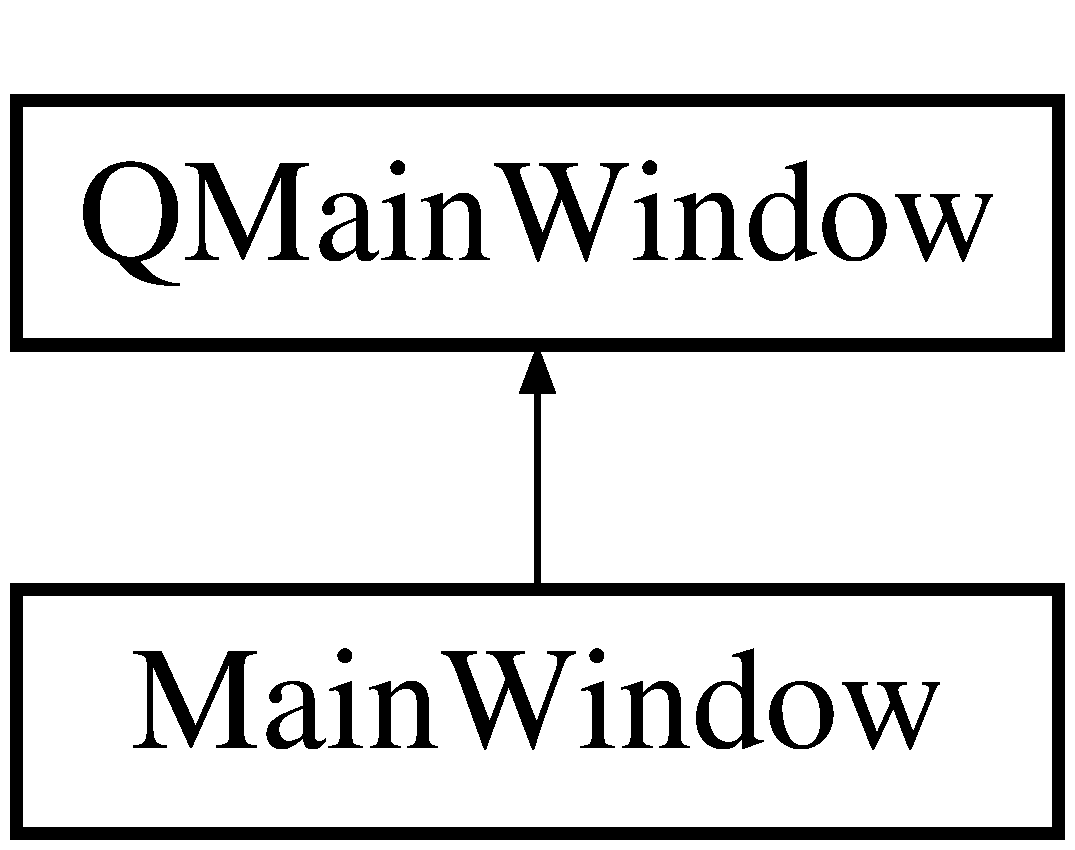
\includegraphics[height=2.000000cm]{class_main_window}
\end{center}
\end{figure}
\subsection*{Public Slots}
\begin{DoxyCompactItemize}
\item 
void \hyperlink{class_main_window_ab2c57d1b4ec7f02e1ed100309e427f93}{s\+\_\+load\+Tiles} ()
\end{DoxyCompactItemize}
\subsection*{Public Member Functions}
\begin{DoxyCompactItemize}
\item 
\hypertarget{class_main_window_a8b244be8b7b7db1b08de2a2acb9409db}{}{\bfseries Main\+Window} (Q\+Widget $\ast$parent=0)\label{class_main_window_a8b244be8b7b7db1b08de2a2acb9409db}

\end{DoxyCompactItemize}


\subsection{Member Function Documentation}
\hypertarget{class_main_window_ab2c57d1b4ec7f02e1ed100309e427f93}{}\index{Main\+Window@{Main\+Window}!s\+\_\+load\+Tiles@{s\+\_\+load\+Tiles}}
\index{s\+\_\+load\+Tiles@{s\+\_\+load\+Tiles}!Main\+Window@{Main\+Window}}
\subsubsection[{s\+\_\+load\+Tiles}]{\setlength{\rightskip}{0pt plus 5cm}void Main\+Window\+::s\+\_\+load\+Tiles (
\begin{DoxyParamCaption}
{}
\end{DoxyParamCaption}
)\hspace{0.3cm}{\ttfamily [slot]}}\label{class_main_window_ab2c57d1b4ec7f02e1ed100309e427f93}
Load tile geometry. Slot function for file/load. Loads texture as well. 

The documentation for this class was generated from the following files\+:\begin{DoxyCompactItemize}
\item 
Main\+Window.\+h\item 
Main\+Window.\+cpp\end{DoxyCompactItemize}

\hypertarget{class_tile}{}\section{Tile Class Reference}
\label{class_tile}\index{Tile@{Tile}}
\subsection*{Public Member Functions}
\begin{DoxyCompactItemize}
\item 
\hypertarget{class_tile_ad7238a794ab70ff75d171810078bc9dd}{}void {\bfseries set\+Num} (int num)\label{class_tile_ad7238a794ab70ff75d171810078bc9dd}

\item 
\hypertarget{class_tile_a437df959501e4730e77650d8a8337597}{}int {\bfseries num} ()\label{class_tile_a437df959501e4730e77650d8a8337597}

\item 
\hypertarget{class_tile_a80c663d21377778108a06a3eddb15475}{}void {\bfseries add\+Vertex} (Q\+Vector2\+D \&)\label{class_tile_a80c663d21377778108a06a3eddb15475}

\item 
\hypertarget{class_tile_a2e323f184c780a57e1a13b99ebe5f04a}{}void {\bfseries set\+Rand\+Color} ()\label{class_tile_a2e323f184c780a57e1a13b99ebe5f04a}

\item 
\hypertarget{class_tile_a0354494ef2c3e38155237628e40ca8db}{}float {\bfseries depth} ()\label{class_tile_a0354494ef2c3e38155237628e40ca8db}

\item 
\hypertarget{class_tile_a4ebdc5646945e0ca9bd09214b0de0d68}{}float {\bfseries angle\+X} ()\label{class_tile_a4ebdc5646945e0ca9bd09214b0de0d68}

\item 
\hypertarget{class_tile_a42d97b17e33adb4a694fb0610315aac5}{}float {\bfseries angle\+Y} ()\label{class_tile_a42d97b17e33adb4a694fb0610315aac5}

\item 
\hypertarget{class_tile_aae18f9c696eef2d0ca491873ca8cad36}{}float {\bfseries angle\+Z} ()\label{class_tile_aae18f9c696eef2d0ca491873ca8cad36}

\item 
\hypertarget{class_tile_a93e6ca9e1a8a2222a9643fd258ca7be6}{}void {\bfseries set\+Depth} (float)\label{class_tile_a93e6ca9e1a8a2222a9643fd258ca7be6}

\item 
\hypertarget{class_tile_ad2c01b4cbacf5ffb1555e32e1cf47989}{}void {\bfseries update\+Depth} (float)\label{class_tile_ad2c01b4cbacf5ffb1555e32e1cf47989}

\item 
\hypertarget{class_tile_a462fbfd2e194bb58e11b585fde37e7e4}{}void {\bfseries update\+Angles} (float, float, float)\label{class_tile_a462fbfd2e194bb58e11b585fde37e7e4}

\item 
\hypertarget{class_tile_ac0d98055b1404168bc0a7fc492300faf}{}Q\+Color {\bfseries color} ()\label{class_tile_ac0d98055b1404168bc0a7fc492300faf}

\item 
\hypertarget{class_tile_a410e2f7ec7fb802f1422a93b8a241af8}{}Q\+Vector2\+D {\bfseries vertex} (int)\label{class_tile_a410e2f7ec7fb802f1422a93b8a241af8}

\item 
\hypertarget{class_tile_a7d5cc53c9a43f117dcedc8f61e78c9af}{}void {\bfseries set\+Centroid} ()\label{class_tile_a7d5cc53c9a43f117dcedc8f61e78c9af}

\item 
\hypertarget{class_tile_a30bde1dc7cfb999f919762312ec02706}{}Q\+Vector2\+D {\bfseries centroid} ()\label{class_tile_a30bde1dc7cfb999f919762312ec02706}

\end{DoxyCompactItemize}


The documentation for this class was generated from the following files\+:\begin{DoxyCompactItemize}
\item 
Tile.\+h\item 
Tile.\+cpp\end{DoxyCompactItemize}

%--- End generated contents ---

% Index
\backmatter
\newpage
\phantomsection
\clearemptydoublepage
\addcontentsline{toc}{chapter}{Index}
\printindex

\end{document}
